\subsection{Tratamiento de ruido}

En la figura~\ref{fig:5a} se muestra la precisión del árbol en función del CF

\begin{figure}
  \centering
  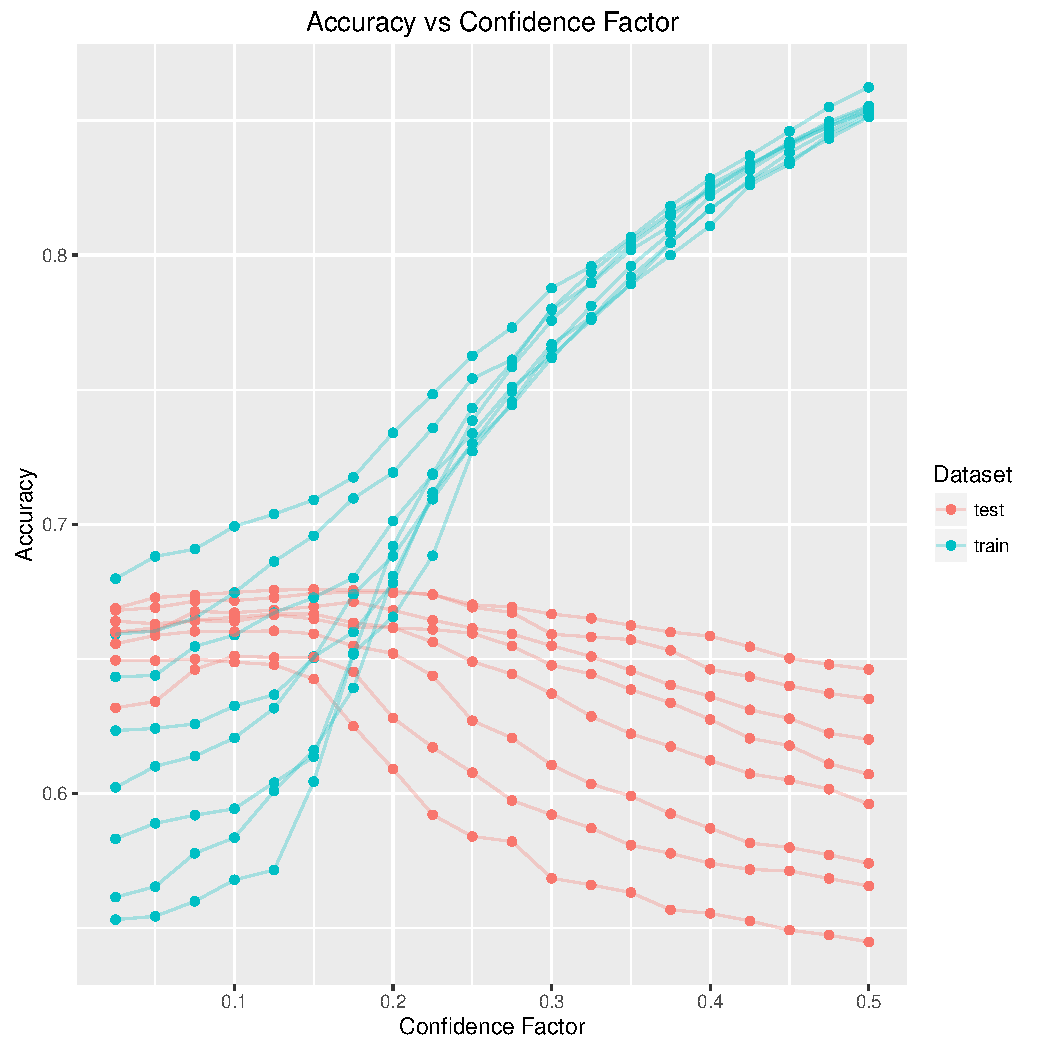
\includegraphics[width = 8cm]{5a.pdf}
  \caption{Accuracy vs CF with noise data}
  \label{fig:5a}
\end{figure}

En la figura~\ref{fig:5b} se muestra el número de hojas en función de porcentaje de datos con ruido.

\begin{figure}
  \centering
  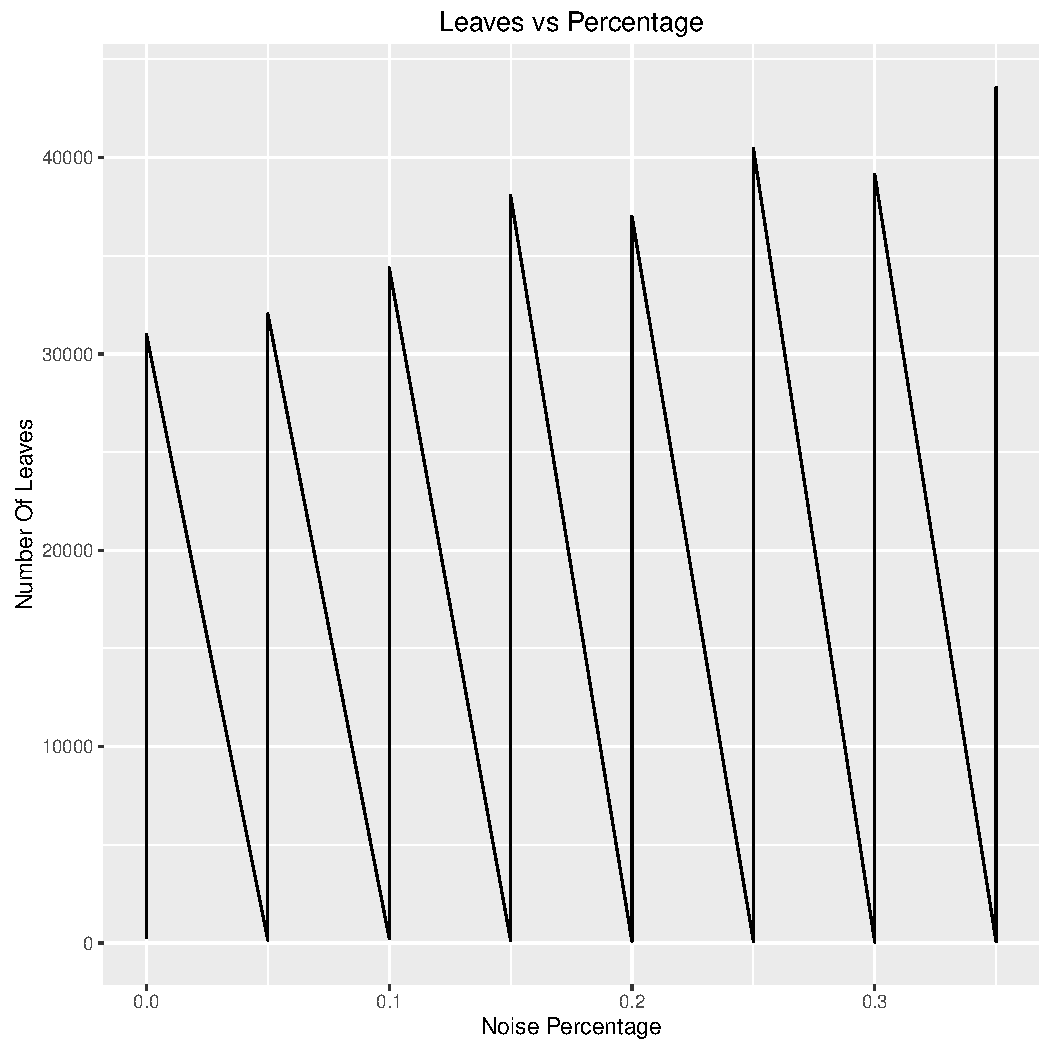
\includegraphics[width = 8cm]{5b.pdf}
  \caption{Leaves vs noice percentage}
  \label{fig:5b}
\end{figure}

En la figura~\ref{fig:5c} se muestra la precisión del árbol en función del porcentaje.

\begin{figure}
  \centering
  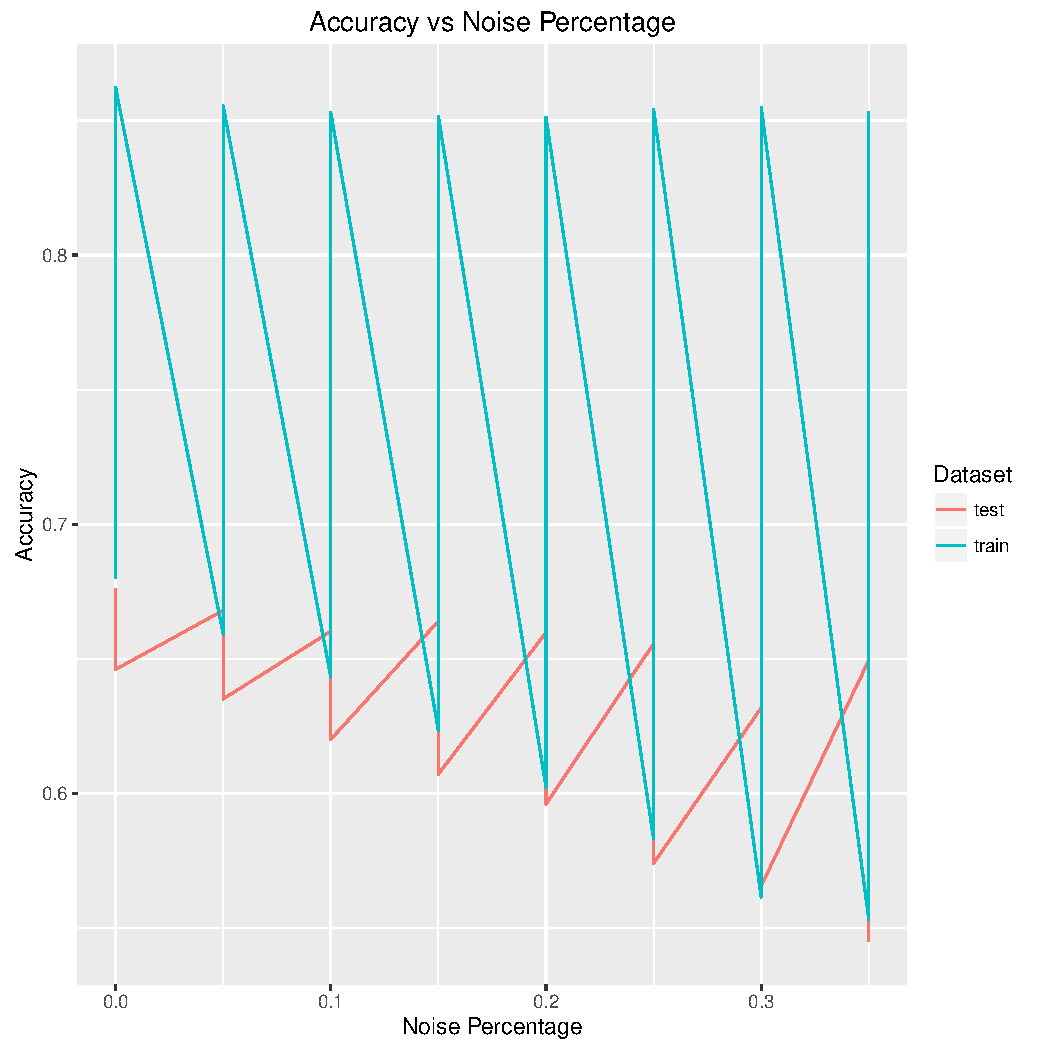
\includegraphics[width = 8cm]{5c.pdf}
  \caption{Accuracy vs noise percentage}
  \label{fig:5c}
\end{figure}

En la figura~\ref{fig:5d} se muestra el porcentaje de ruido en función del CF.

\begin{figure}
  \centering
  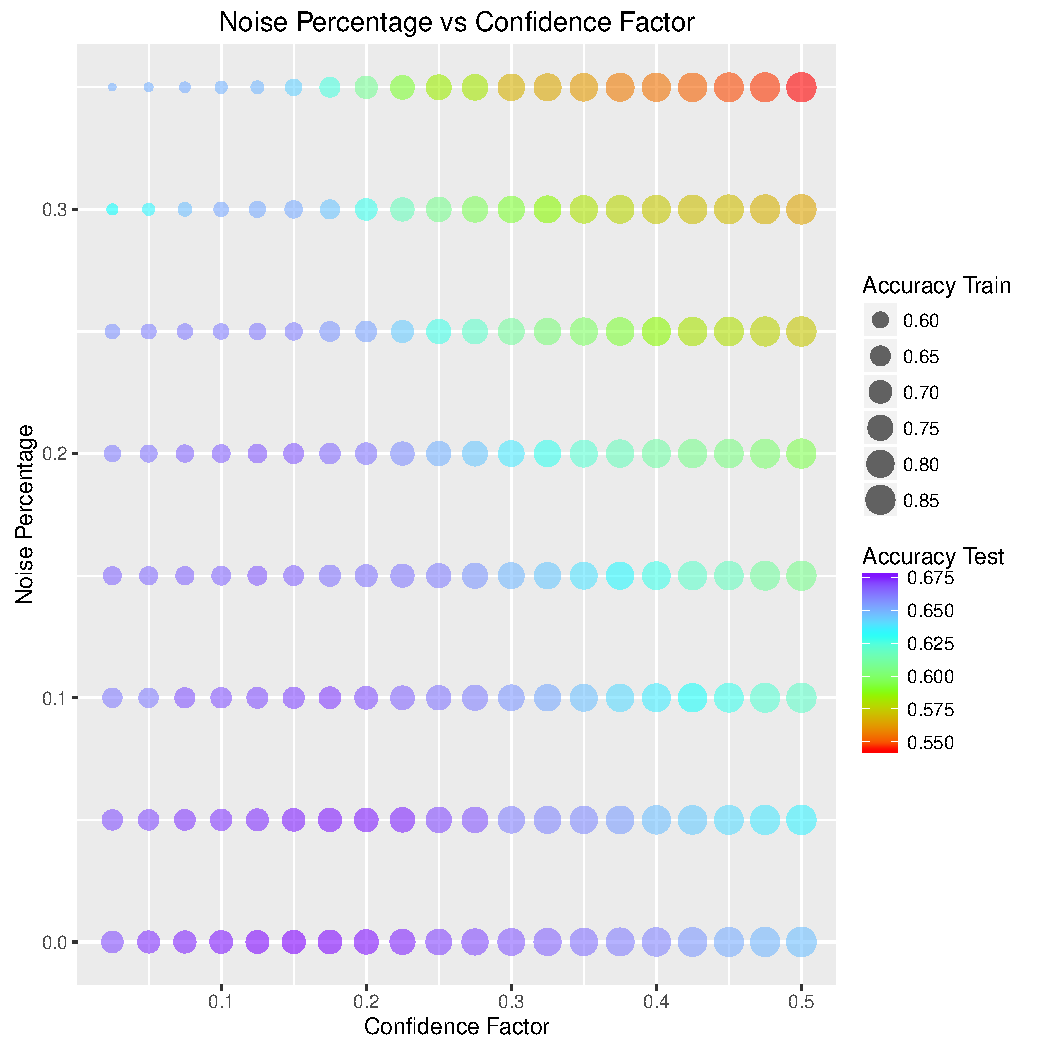
\includegraphics[width = 8cm]{5d.pdf}
  \caption{Noise percentage vs CF}
  \label{fig:5d}
\end{figure}

